\documentclass{article}

\def\npart {II}
\def\nyear {2017}
\def\nterm {Lent}
\def\nlecturer{Dr R.\ Camina}
\def\ncourse{Coding and Cryptography}
\ifx \nauthor\undefined
  \def\nauthor{Bhavik Mehta}
\else
\fi

\author{Based on lectures by \nlecturer \\\small Notes taken by \nauthor}
\date{\nterm\ \nyear}
\title{Part \npart\ -- \ncourse}

\usepackage[utf8]{inputenc}
\usepackage{amsmath}
\usepackage{amsthm}
\usepackage{amssymb}
\usepackage{enumerate}
\usepackage{mathtools}
\usepackage{graphicx}
\usepackage[dvipsnames]{xcolor}
\usepackage{tikz}
\usepackage{wrapfig}
\usepackage{centernot}
\usepackage{float}
\usepackage{braket}
\usepackage[hypcap=true]{caption}
\usepackage{enumitem}
\usepackage[colorlinks=true, linkcolor=mblue]{hyperref}
\usepackage[nameinlink,noabbrev]{cleveref}
\usepackage{nameref}
\usepackage[margin=1.5in]{geometry}

% Theorems
\theoremstyle{definition}
\newtheorem*{aim}{Aim}
\newtheorem*{axiom}{Axiom}
\newtheorem*{claim}{Claim}
\newtheorem*{cor}{Corollary}
\newtheorem*{conjecture}{Conjecture}
\newtheorem*{defi}{Definition}
\newtheorem*{eg}{Example}
\newtheorem*{ex}{Exercise}
\newtheorem*{fact}{Fact}
\newtheorem*{law}{Law}
\newtheorem*{lemma}{Lemma}
\newtheorem*{notation}{Notation}
\newtheorem*{prop}{Proposition}
\newtheorem*{question}{Question}
\newtheorem*{rrule}{Rule}
\newtheorem*{thm}{Theorem}
\newtheorem*{assumption}{Assumption}

\newtheorem*{remark}{Remark}
\newtheorem*{warning}{Warning}
\newtheorem*{exercise}{Exercise}

% \newcommand{\nthmautorefname}{Theorem}

\newtheorem{nthm}{Theorem}[section]
\newtheorem{nlemma}[nthm]{Lemma}
\newtheorem{nprop}[nthm]{Proposition}
\newtheorem{ncor}[nthm]{Corollary}
\newtheorem{ndef}[nthm]{Definition}

% Special sets
\newcommand{\C}{\mathbb{C}}
\newcommand{\N}{\mathbb{N}}
\newcommand{\Q}{\mathbb{Q}}
\newcommand{\R}{\mathbb{R}}
\newcommand{\Z}{\mathbb{Z}}

\newcommand{\abs}[1]{\left\lvert #1\right\rvert}
\newcommand{\norm}[1]{\left\lVert #1\right\rVert}
\renewcommand{\vec}[1]{\boldsymbol{\mathbf{#1}}}

\let\Im\relax
\let\Re\relax

\DeclareMathOperator{\Im}{Im}
\DeclareMathOperator{\Re}{Re}
\DeclareMathOperator{\id}{id}

\definecolor{mblue}{rgb}{0., 0.05, 0.6}


% preamble
\usepackage{tikz}
\usepackage{pgfplots}
\usetikzlibrary{arrows,decorations.pathmorphing,decorations.markings,positioning}
\renewcommand{\thesection}{\Roman{section}}
\DeclarePairedDelimiter{\ceil}{\lceil}{\rceil}
\pgfplotsset{width=7cm}
% and here we go!

\begin{document}
\maketitle
\tableofcontents

\section*{Introduction to communication channels and coding}
For example, given a message $m$=`Call me!' which we wish to send by email, first encode as binary strings using ASCII.
So, $f(C) = 1000011, f(a) = 1100001$, and $f^*(m) = 1000011\ 1100001 \dots 0100001$.
% picture
\tikzstyle{block} = [rectangle, draw, fill=YellowOrange!20,
    text width=4em,
    text centered,
    minimum height=2em
    ]
\begin{center}
    \begin{tikzpicture}[node distance=3cm]
        \node (s) at (0, 0) [block] {source};
        % this is kind of horrible but it works :/
        \node (e) at (3, 0) [block] {encoder};
        \node (d) at (8, 0) [block] {decoder};
        \node (r) at (11, 0) [block] {receiver};
        \draw [->, shorten > =0.1em, thick] (s) -- (e);
        \draw [->, shorten > =0.1em, thick, decorate, decoration={amplitude=1.5mm,
            segment length=10mm,
            snake, post length=1mm}] (e) -- (d)
            node [above=0.5em,align=center,midway] {channel}
            node [below=0.5em,align=center,midway,color=red] {errors};

        \draw [->, shorten > =0.1em, thick] (d) -- (r);
    \end{tikzpicture}
\end{center}

\textbf{Basic problem:} Given a source and a channel (described probabilistically) we aim to design an encoder and a decoder in order to transmit information both economically and reliably (coding) and maybe also to preserve privacy (cryptography).

\begin{eg}
\leavevmode
\begin{itemize}
    \item `economically'
    Morse code: common letters have shorter codewords:
    % A .-, E ., Q --.--
    \item `reliably'
    Every book has an ISBN of form $a_1 a_2 \dotsc a_{10}$ where $a_i \in \{0, 1, \dotsc, 9\}$ for $1 \leq i \leq 9$, $a_{10} \in \{0, 1, \dotsc, 9, X\}$ such that
    \begin{equation*}
        10 a_1 + 9 a_2 + \dotsc + a_{10} \equiv 0 \pmod{11}
    \end{equation*}
    so errors can be detected (but not corrected).
    Similarly a 13-digit ISBN has
    \begin{equation*}
        x_1 + 3 x_2 + x_3 + 3 x_4 + \dotsc + 3 x_{12} + x_{13} \equiv 0 \pmod{10}
    \end{equation*}
    for $0 \leq x_i \leq 10$, doesn't necessarily spot transpositions.
\item `preserve privacy' e.g. RSA.
\end{itemize}
\end{eg}

A \textbf{communication channel} takes letters from an input alphabet $\Sigma_1 = \{a_1, \dotsc, a_r\}$ and emits letters form an output alphabet $\Sigma_2 = \{b_1, \dotsc, b_s\}$.

A channel is determined by the probabilities
\begin{equation*}
    P(y_1 \dotsc y_k \text{ received} \mid x_1 \dotsc x_k \text{ sent})
\end{equation*}

\begin{defi}[Discrete memoryless channel]\hypertarget{def:dmc}
    A \textbf{discrete memoryless channel} (DMC) is a channel for which
    \begin{equation*}
        P_{ij} = P(b_j \text{ received} \mid a_i \text{ sent})
    \end{equation*}
    is the same each time the channel is used and is independent of all past and future uses.
\end{defi}

The channel matrix is the $r \times s$ matrix with entries $p_{ij}$ (note the rows sum to 1).

\begin{eg}
    Binary Symmetric Channel (BSC) has $\Sigma_1 = \Sigma_2 = \{0, 1\}$, $0 \leq p \leq 1$:
    \begin{center}
        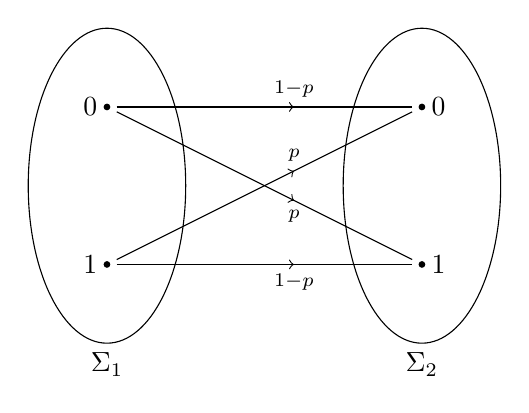
\begin{tikzpicture}
            \draw (-2, 0) circle [x radius=1cm, y radius=2cm] node [below=2cm] {$\Sigma_1$};
            \draw ( 2, 0) circle [x radius=1cm, y radius=2cm] node [below=2cm] {$\Sigma_2$};

            \node (0l) at (-2, 1) {};
            \node (1l) at (-2,-1) {};

            \node (0r) at (2, 1) {};
            \node (1r) at (2,-1) {};

            \filldraw (0l) circle (1pt) node [left] {0};
            \filldraw (1l) circle (1pt) node [left] {1};
            \filldraw (0r) circle (1pt) node [right] {0};
            \filldraw (1r) circle (1pt) node [right] {1};

            \begin{scope}[decoration={
                markings,
                mark=at position 0.6 with {\arrow{>}}}
                ]
                \draw[postaction={decorate}] (0l) -- (0r)
                    node [above,align=center,pos=0.6] {$\scriptstyle 1-p$};
                \draw[postaction={decorate}] (0l) -- (1r)
                    node [below,align=center,pos=0.6] {$\scriptstyle p$};
                \draw[postaction={decorate}] (1l) -- (0r)
                    node [above,align=center,pos=0.6] {$\scriptstyle p$};
                \draw[postaction={decorate}] (1l) -- (1r)
                    node [below,align=center,pos=0.6] {$\scriptstyle 1-p$};
            \end{scope}
        \end{tikzpicture}
    \end{center}
    with channel matrix
    \begin{equation*}
        \begin{pmatrix}
            1-p & p \\ p & 1-p
        \end{pmatrix}
    \end{equation*}
    i.e. $p$ is the probability a symbol is mistransmitted.


    Another example is given by the Binary Erasure channel, $\Sigma_1 \{0, 1\}$, $\Sigma_2 = \{0, 1, *\}$ and $0 \leq p \leq 1$.
    \begin{center}
        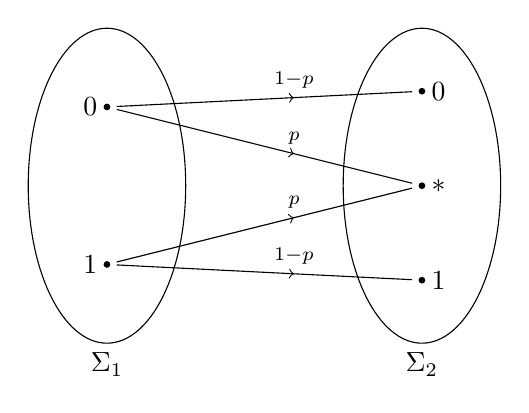
\begin{tikzpicture}
            \draw (-2, 0) circle [x radius=1cm, y radius=2cm] node [below=2cm] {$\Sigma_1$};
            \draw ( 2, 0) circle [x radius=1cm, y radius=2cm] node [below=2cm] {$\Sigma_2$};

            \node (0l) at (-2, 1) {};
            \node (1l) at (-2,-1) {};

            \node (0r) at (2, 1.2) {};
            \node (*r) at (2,   0) {};
            \node (1r) at (2,-1.2) {};

            \filldraw (0l) circle (1pt) node [left] {0};
            \filldraw (1l) circle (1pt) node [left] {1};
            \filldraw (0r) circle (1pt) node [right] {0};
            \filldraw (*r) circle (1pt) node [right] {$*$};
            \filldraw (1r) circle (1pt) node [right] {1};

            \begin{scope}[decoration={
                markings,
                mark=at position 0.6 with {\arrow{>}}}
                ]
                \draw[postaction={decorate}] (0l) -- (0r)
                    node [above,align=center,pos=0.6] {$\scriptstyle 1-p$};
                \draw[postaction={decorate}] (0l) -- (*r)
                    node [above,align=center,pos=0.6] {$\scriptstyle p$};
                \draw[postaction={decorate}] (1l) -- (*r)
                    node [above,align=center,pos=0.6] {$\scriptstyle p$};
                \draw[postaction={decorate}] (1l) -- (1r)
                    node [above,align=center,pos=0.6] {$\scriptstyle 1-p$};
            \end{scope}
        \end{tikzpicture}
    \end{center}
    with channel matrix
    \begin{equation*}
        \begin{pmatrix}
            1-p & p & 0 \\
            0 & p & 1-p
        \end{pmatrix}
    \end{equation*}
    i.e. $p$ is the probability a symbol can't be read.
\end{eg}

Informally, a channel's capacity is the highest rate at which information can be reliably transmitted over the channel.
Rate refers to units of information per unit time, which we want to be high. Similarly, reliably means we want an arbitrarily small error probability.

\clearpage
\section{Noiseless Coding}
\begin{notation}
    For $\Sigma$ an alphabet, let $\Sigma^* = \bigcup_{n \geq 0} \Sigma^n$ be the set of all finite strings of elements of $\Sigma$.
\end{notation}
If $x = x_1 \dotsc x_r$, $y = y_1 \dotsc y_s$ are strings from $\Sigma$, write $xy$ for the concatenation $x_1 \dotsc x_r y_1 \dotsc y_s$.
Further, $\abs{x_1 \dotsc x_r y_1 \dotsc y_s} = r+s$, the length of the string.
\begin{defi}[Code]\hypertarget{def:code}
    Let $\Sigma_1, \Sigma_2$ be two alphabets. A \textbf{code} is a function $f: \Sigma_1 \to \Sigma_2^*$. The strings $f(x)$ for $x \in \Sigma_1$ are called \textbf{codewords}.
\end{defi}
\begin{eg}
    \leavevmode
    \begin{enumerate}[label=\arabic*)] % 1)
        \item
            \hypertarget{ex:greekFire}{Greek fire} \hyperlink{def:code}{code}:
            \begin{align*}
                \Sigma_1 &= \{\alpha, \beta, \gamma, \dotsc, \omega\} \quad \text{ 24 letters} \\
                \Sigma_2 &= \{1, 2, 3, 4, 5\}
            \end{align*}
            so, $\alpha \mapsto 11, \beta \mapsto 12, \dotsc, \omega \mapsto 54$.
        \item
            $\Sigma_1 = $ \{all words in the dictionary\}, and $\Sigma_2 = \{A, B, \dotsc, Z, [space]\}$ % add space symbol
            and $f$=`spell the word and a space'\hypertarget{ex:comma-code}.
    \end{enumerate}
\end{eg}
We send a message $x_1, \dotsc, x_n \in \Sigma_1^*$ as $f(x_1) f(x_2) \dotsm f(x_n) \in \Sigma_2^*$ i.e. extend $f$ to $f^* : \Sigma_1^* \to \Sigma_2^*$.

\begin{defi}[Decipherable]\hypertarget{def:decipherable}
    A \hyperlink{def:code}{code} $f$ is \textbf{decipherable} if $f^*$ is injective, i.e. every string from $\Sigma_2$ arises from at most one message.
    Clearly we need $f$ injective, but this is not enough.
\end{defi}

% Lecture 2

\begin{eg}
    Take $\Sigma_1 = \{1, 2, 3, 4\}$, $\Sigma_2 = \{0, 1\}$ with
    \begin{equation*}
        f(1) = 0, f(2) = 1, f(3) = 00, f(4) = 01
    \end{equation*}
    $f$ injective but $f^*(312) = 0001 = f^*(114)$ so $f^*$ not \hyperlink{def:decipherable}{decipherable}.
\end{eg}

\begin{notation}
    If $\abs{\Sigma_1} = m$, $\abs{\Sigma_2} = a$, then we say $f$ is an $a$-ary code of size $m$. (If $a=2$ we say binary).
\end{notation}
\begin{aim}
    Construct \hyperlink{def:decipherable}{decipherable} \hyperlink{def:code}{codes} with short word lengths.
\end{aim}

Provided $f: \Sigma_1 \to \Sigma_2^*$ is injective, the following codes are always decipherable.
\begin{enumerate}[label=(\roman*)]
    \item A \textbf{block code} is a code with all codewords of the same length (e.g. \hyperlink{eg:greekFire}{Greek fire code}).
    \item In a \textbf{comma code}, we reserve one letter from $\Sigma_2$ that is only used to signal the end of the codeword (e.g. \hyperlink{ex:comma-code}{Example 2 above}).
    \item A \hypertarget{def:prefixFreeCode}{\textbf{prefix-free code}} is a code where no codeword is a prefix of another (if $x, y \in \Sigma_2^*$, $x$ is a prefix of $y$ if $y=xz$ for some $z \in \Sigma_2^*$.)
\end{enumerate}

\begin{remark}(i) and (ii) are special cases of (iii).
\end{remark}

Prefix-free codes are also known as \textbf{instantaneous codes} (i.e. a word can be recognised as soon as it is complete) or \textbf{self-punctuating codes}.

% thm 1.1
\begin{nthm}[Kraft's inequality]\label{thm:kraft}
    Let $\abs{\Sigma_1} = m, \abs{\Sigma_2} = a$. A prefix-free code $f: \Sigma_1 \to \Sigma_2^*$ with word lengths $s_1, \dotsc, s_m$ exists iff
    \begin{equation*}
        \sum_{i = 1}^m a^{-s_i} \leq 1
    \end{equation*}
\end{nthm}

\begin{proof}
    $(\Rightarrow)$ Consider an infinite tree where each has a descendant, labelled by the elements of $\Sigma_2$. Each codeword corresponds to a node, the path from the root to this node spelling out the codeword.
    For example,
    \begin{center}
        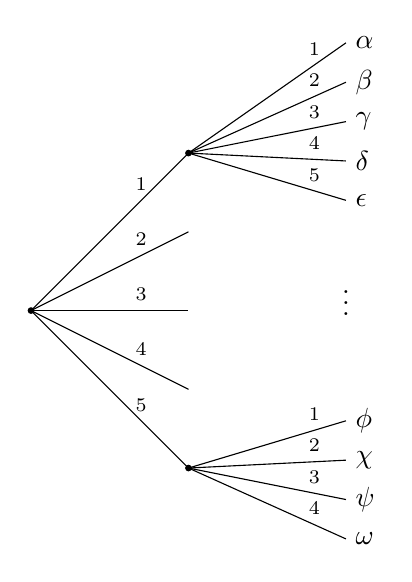
\begin{tikzpicture}[scale=2]
            \filldraw (0, 0) circle (0.5pt);
            \filldraw (1, 1) circle (0.5pt);
            \filldraw (1,-1) circle (0.5pt);
            \foreach \x in {1,...,5}{
                \pgfmathsetmacro\a{(3-\x)/2.0}
                \pgfmathsetmacro\b{(3-\x)/4.0 + 1.2}
                \draw (0, 0) --(1, \a) node[pos=0.7, above] {$\scriptstyle \x$};
                \draw (1, 1) -- (2, \b) node[pos=0.8, above] {$\scriptstyle \x$};
            };
            \foreach \x in {1,...,4}{
                \pgfmathsetmacro\c{(3-\x)/4.0 - 1.2}
                \draw (1, -1) -- (2, \c) node[pos=0.8, above] {$\scriptstyle \x$};
            };
            \node at (2, 0.1) {$\vdots$};
            \node [right] at (2, 1.7) {$\alpha$};
            \node [right] at (2, 1.45) {$\beta$};
            \node [right] at (2, 1.2) {$\gamma$};
            \node [right] at (2, 0.95) {$\delta$};
            \node [right] at (2, 0.7) {$\epsilon$};

            \node [right] at (2, -0.7) {$\phi$};
            \node [right] at (2, -0.95) {$\chi$};
            \node [right] at (2, -1.2) {$\psi$};
            \node [right] at (2, -1.45) {$\omega$};
        \end{tikzpicture}
    \end{center}
    Assuming $f$ is prefix-free, no codeword is the ancestor of any other. Now view the tree as a network with water being pumped in at a constant rate and dividing the flow equally at each node.

    The total amount of water we can extract at the codewords is $\sum_{i=1}^m a^{-s_i}$, which is therefore $\leq 1$.

    $(\Leftarrow)$ Conversely, suppose we can construct a prefix-free code with word lengths $s_1, \dotsc, s_m$ wlog $s_1 \leq s_2 \leq \dotsb \leq s_m$.
    We pick codewords of lengths $s_1, s_2, \dotsc$ sequentially ensuring previous codewords are not prefixes.
    Suppose there is no valid choice for the $r$th codeword.
    Then reconstructing the tree as above gives $ \sum_{i=1}^{r-1} a^{-s_i} = 1 $, contradicting our assumption.
    So we can construct a prefix-free code. (There is a more algebraic proof in Welsh.)
\end{proof}

\begin{nthm}[McMillan]
    Every decipherable code satisfies Kraft's inequality.
\end{nthm}

\begin{proof}(Karush)
    Let $f: \Sigma_1 \to \Sigma_2^*$ be a decipherable code with word lengths $s_1, \dotsc, s_m$, let $s = \max_{1 \leq i \leq m} s_i$.
    Let $r \in \N$
    \begin{equation*}
        \left(\sum_{i=1}^m a^{-s_i}\right)^r = \sum_{l=1}^{rs} b_l a^{-l}
    \end{equation*}
    where $b_l$ is the \# of ways of choosing $r$ codewords of total length $l$. $f$ decipherable $\implies b_l \leq \abs{\Sigma_2}^l = a^l$.

    Thus \begin{align*}\left(\sum_{i=1}^m a^{-s_i}\right)^r \leq \sum_{l=1}^{rs} a^l a^{-l} = rs \\
    \implies \sum_{i=1}^m a^{-s_i} \leq (rs)^{\frac{1}{r}} \to 1 \text{ as } r \to \infty.
    \end{align*}
    (As $\frac{\log r + \log s}{r} \to 0$ as $r \to \infty$).
    \begin{equation*}
        \therefore \sum_{i=1}^m a^{-s_i} \leq 1.
    \end{equation*}
\end{proof}

\begin{eg}
    \leavevmode
    \begin{enumerate}[label=\arabic*.]
        \item Suppose $p_1 = p_2 = p_3 = p_4 = \frac{1}{4}$. We identify $\{x_1, x_2, x_3, x_4\}$ with \{HT, HT, TH, TT\}. Then $H(X) = 2$.
        \item Take $(p_1, p_2, p_3, p_4) = (\frac{1}{2}, \frac{1}{4}, \frac{1}{8}, \frac{1}{8})$.
            \begin{center}
                \begin{tikzpicture}[xscale=1.8, yscale=0.8]
                    \draw (0,0) -- (1,1);
                    \draw (0,0) -- (1, -1);
                    \draw (1, -1) -- (2, 0);
                    \draw (1, -1) -- (2, -2);
                    \draw (2, -2) -- (3, -1);
                    \draw (2, -2) -- (3, -3);
                    \node [right] at (1, 1) {$\frac{1}{2}$};
                    \node [right] at (2, 0) {$\frac{1}{4}$};
                    \node [right] at (3, -1) {$\frac{1}{8}$};
                    \node [right] at (3, -3) {$\frac{1}{8}$};
                \end{tikzpicture}
            \end{center}
            So example 1 is more random than example 2.
    \end{enumerate}
\end{eg}

\begin{defi}[Entropy]\hypertarget{def:entropy}
    The entropy of $X$:
    \begin{equation*}
        H(X) = H(p_1, \dotsc, p_n) = -\sum_{i=1}^n p_i \log p_i
    \end{equation*}
    where, in this course, $\log = \log_2$.
\end{defi}

\begin{remark}
    \leavevmode
    \begin{enumerate}[label=(\roman*)]
        \item If $p_i = 0$, we take $p_i \log p_i=0$.
        \item $H(x) \geq 0$.
    \end{enumerate}
\end{remark}

\begin{cor}
    A decipherable code with prescribed word lengths exists iff there exists a prefix-free code with the same word lengths.
\end{cor}
So we can restrict our attention to prefix-free codes.

\subsection{Mathematical Entropy}
\hyperlink{def:entropy}{Entropy} is a measure of `randomness' or `uncertainty'.
Consider a random variable $X$ taking values $x_1, \dotsc, x_n$ with probability $p_1, \dotsc, p_n$ ($\sum p_i = 1, 0 \leq p_i \leq 1$).
The entropy $H(X)$ is roughly speaking the expected number of tosses of a fair coin needed to simulate $X$ (or the expected number of yes/no questions we need to ask in order to establish the value of $X$).

% Lecture 3
\begin{eg}
    We toss a biased coin, $P(\text{heads}) = p, P(\text{tails}) = 1-p$. Write $H(p) = H(p, 1-p) = -p \log p - (1-p) \log (1-p)$.
    If $p=0$ or $1$, the outcome is certain and so entropy=0. Entropy is maximal where $p=\frac{1}{2}$, i.e. a fair coin.

    \begin{center}
        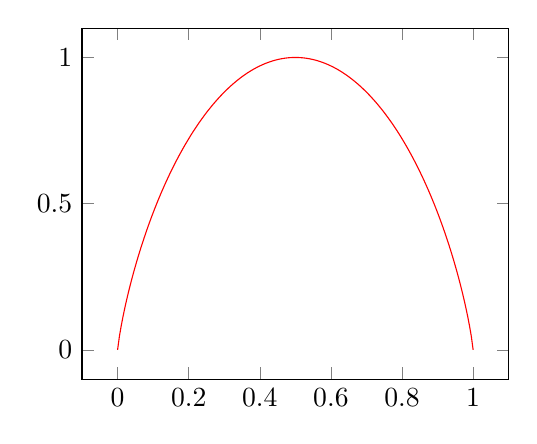
\begin{tikzpicture}
            \begin{axis}[]
            \addplot [
            red,
            domain=0:1,
            samples=201,
            ]
            {-x*log2(x) - (1-x)*log2(1-x)};
            \end{axis}
        \end{tikzpicture}
    \end{center}
\end{eg}

Note the \hyperlink{def:entropy}{entropy} can also be viewed as the expected value of the information of $X$, where information is given by $I(X=x) = -\log_2 P(X=x)$.
For example, if a coin always lands heads we gain no information from tossing the coin.
The entropy is the average amount of information conveyed by a random variable $X$.

\begin{nlemma}[Gibbs' Inequality]\label{lem:gibbs}
    Let $p_1, \dotsc, p_n$ and $q_1, \dotsc, q_n$ be probability distributions. Then
    \begin{equation*}
        -\sum p_i \log p_i \leq -\sum p_i \log q_i
    \end{equation*}
    with equality iff $p_i = q_i$.
\end{nlemma}
\begin{proof}
    Since $\log x = \frac{\ln x}{\ln 2}$ it suffices to prove the inequality with $\log$ replaced with $\ln$.
    Note $\ln x \leq x - 1$, equality iff $x=1$.
    % graph x-1 and ln x
    Let $I = \set{1 \leq i \leq n | p_i \neq 0}$
    \begin{align*}
        \ln \frac{q_i}{p_i} &\leq \frac{q_i}{p_i} - 1 \quad \forall i \in I \\
        \sum_{i \in I} p_i \ln \frac{q_i}{p_i} &\leq \sum q_i - \underbrace{\sum p_i}_{=1} \leq 0 \\
        \implies -\sum_{i \in I} p_i \ln p_i &\leq -\sum_{i \in I} p_i \ln q_i \\
        \implies -\sum_{i =1}^n p_i \ln p_i &\leq -\sum_{i =1}^n p_i \ln q_i \\
    \end{align*}
    If equality holds then $\frac{q_i}{p_i} = 1$ $\forall i \in I$. So, $\sum_{i \in I} q_i = 1$ and hence $p_i = q_i$ for $1 \leq i \leq n$.
\end{proof}

\begin{cor}
    $H(p_1, \dotsc, p_n) \leq \log n$ with equality iff $p_1 = p_2 = \dotsb = p_n = \frac{1}{n}$.
\end{cor}
\begin{proof}
    Take $q_1 = q_2 = \dotsc = q_n = \frac{1}{n}$ in previous lemma.
\end{proof}

Suppose we have two alphabets $\Sigma_1, \Sigma_2$ with $\abs{\Sigma_1} = m$ and $\abs{\Sigma_2} = a$, for $m \geq 2$ and $a \geq 2$.
We model the source as a sequence of random variables $X_1, X_2, \dotsc$ taking values in $\Sigma_1$.
\begin{defi}[Memoryless source]\hypertarget{def:memoryless}
    A \textbf{Bernoulli} or \textbf{memoryless} source is a sequence of independently, identically distributed random variables.
\end{defi}
That is, for each $\mu \in \Sigma_1$, $P(X_i = \mu)$ is independent of $i$ and independent of all past and future symbols emitted. Thus
\begin{equation*}
    P(X_1= x_1, X_2 = x_2, \dotsc, X_k = x_k) = \prod_{i = 1}^k P(X_i = x_i)
\end{equation*}
Let $\Sigma_1 = \{\mu_1, \dotsc, \mu_n\}$, $p_i = P(X=\mu_i)$ (assume $p_i > 0$).
\begin{defi}[Expected word length]\hypertarget{def:ewl}
    The \textbf{expected word length} of a code $f: \Sigma_1 \to \Sigma_2^*$ with word lengths $s_1, \dotsc, s_m$ is $E(S) = \sum_{i=1}^m p_i s_i$.
\end{defi}

\begin{defi}[Optimal code]\hypertarget{def:optCode}
    A \hyperlink{def:code}{code} $f:\Sigma_1 \to \Sigma_2^*$ is \textbf{optimal} if it has the shortest possible \hyperlink{def:ewl}{expected word length} among \hyperlink{def:decipherable}{decipherable} codes.
\end{defi}
\begin{nthm}[Shannon's Noiseless Coding Theorem]
    The minimum \hyperlink{def:ewl}{expected word length} of a \hyperlink{def:decipherable}{decipherable code} $f: \Sigma_1 \to \Sigma_2^*$ satisfies
    \begin{equation*}
        \frac{H(X)}{\log a} \leq E(S) < \frac{H(X)}{\log a} + 1
    \end{equation*}
\end{nthm}
\begin{proof}
    The lower bound is given by combining \nameref{lem:gibbs} and \nameref{thm:kraft}.
    Let $q_i = \frac{a^{-s_i}}{c}$ where $c = \sum a^{-s_i} \leq 1$ by \nameref*{thm:kraft}.
    Note $\sum q_i = 1$.
    \begin{align*}
        H(X) = -\sum p_i \log p_i &\leq -\sum_i p_i \log q_i \\
                                  &= \sum p_i (s_i \log a + \log c) \\
                                  &= \left(\sum p_i s_i\right) \log a + \underbrace{\log c}_{\leq 0} \leq E(S) \log a\\
        \implies \frac{H(X)}{\log a} &\leq E(S)
    \end{align*}
    We get equality $\iff p_i = a^{-s_i}$ for some integers $s_i$.
    For the upper bound put
    \begin{equation*}
        s_i = \ceil{-\log_a p_i}
    \end{equation*}
    where $\ceil{x}$ means least integer $\geq x$.

    We have
    \begin{gather*}
        - \log_a p_i \leq s_i < - \log_a p_i + 1 \\
        \implies a^{-s_i} \leq p_i \implies \sum a^{-s_i} \leq \sum p_i \leq 1.
    \end{gather*}
    So by \cref{thm:kraft}, $\exists$ a prefix-free code with word lengths $s_1, \dotsc, s_m$.
    Also,
    \begin{align*}
        E(S) &= \sum p_i s_i \\
             &< p_i (- \log_a p_i + 1) \\
             &= \frac{H(X)}{\log a} + 1
    \end{align*}
\end{proof}
\begin{remark}
    The lower bound holds for all decipherable codes.
\end{remark}

\subsubsection*{Shannon-Fano coding}
Follows from above proof.
Set $s_i = \ceil{-\log_a p_i}$ and construct a prefix-free code with word lengths $s_1, \dotsc, s_m$ by taking the $s_i$ in increasing order ensuring that previous codewords are not prefixes.
The Kraft inequality ensures there is enough room.
\begin{eg}
    Suppose $\mu_1, \dotsc, \mu_5$ are emitted with probabilities $0.4, 0.2, 0.2, 0.1, 0.1$.

    A \hypertarget{ex:shannonfano1}{possible Shannon-Fano} code (with $a=2$, $\Sigma_2 = \{0, 1\}$) has
    \begin{center}
    \begin{tabular}{c c c}
        $p_i$ & $\ceil{-\log_2 p_i}$ & \\
        \hline
        0.4 & 2 & 00 \\
        0.2 & 3 & 010 \\
        0.2 & 3 & 100 \\
        0.1 & 4 & 1100 \\
        0.1 & 4 & 1110
    \end{tabular}
    \end{center}
    This has \hyperlink{def:ewl}{expected word length}
    \begin{align*}
        &= 2 \times 0.4 + 3 \times 0.2 + 3 \times 0.2 + 4 \times 0.1 + 4 \times 0.1 \\
        &= 2.8.
    \end{align*}
    compare $H(X) \approx 2.12$.
\end{eg}

\subsubsection*{Huffman coding}
For simplicity, take $a=2$.
Take $\Sigma_1=\{\mu_1, \dotsc, \mu_m\}$ with $p_i = P(X = \mu_i)$. Without loss of generality, $p_1 \geq p_2 \geq \dotsb \geq p_m$.
Huffman coding is defined inductively.

If $m=2$, assign codewords $0$ and $1$. If $\mu > 2$, find a Huffman coding in the case of messages $\mu_1, \mu_2, \dotsc, \nu$, with probabilities $p_1, p_2, \dotsc, p_{m-1} + p_m$.

Append $0$ (resp, $1$) to the codeword for $\nu$ to give a codeword for $\mu_{m-1}$ (resp, $\mu_m$).

\begin{remark}
    \leavevmode
    \begin{enumerate}[label=\roman*)]
        \item This construction gives a prefix-free code.
        \item We exercise some choice when some of the $p_i$ are equal. So Huffman codes are not unique.
    \end{enumerate}
\end{remark}

\begin{eg}
    Use the same \hyperlink{ex:shannonfano1}{example probabilities} as earlier. \\
    (diagram of example) \\
    So $\{1, 00, 011, 0101, 0100\}$ is the prefix-free code constructed. The \hyperlink{def:ewl}{expected word length} is:
    \begin{align*}
        &= 1 \times 0.4 + 2 \times 0.2 + 2 \times 0.2 + 4 \times 0.1 + 4 \times 0.1 \\
        &= 0.4 + 0.4 + 0.6 + 0.4 + 0.4\\
        &= 2.2.
    \end{align*}
    This is better than Shannon-Fano, which gave 2.8.
\end{eg}

\begin{nthm}\label{thm:huffOpt}
    Huffman coding is \hyperlink{def:optCode}{optimal}.
\end{nthm}
\begin{nlemma}
    Suppose we have $\mu_1, \dotsc, \mu_m \in \Sigma_1$ emitted with probabilities $p_1, \dotsc, p_m$.
    Let $f$ be an \hyperlink{def:optCode}{optimal} \hyperlink{def:prefixFreeCode}{prefix-free} \hyperlink{def:code}{code}, with word lengths $s_1, \dotsc, s_m$.
    Then
    \begin{enumerate}[label=\roman*)]
        \item If $p_i > p_j$, then $s_i \leq s_j$.
        \item $\exists$ two codewords of maximal length which are equal up to the last digit.
    \end{enumerate}
\end{nlemma}

\begin{proof}
    \leavevmode
    \begin{enumerate}[label=\roman*)]
        \item If not, then swap the $i$th and $j$th \hyperlink{def:codewords}{codewords}.
            This decreases the \hyperlink{def:ewl}{expected word length}, contradicting $f$ \hyperlink{def:optCode}{optimal}.
        \item If not, then either only one codeword of maximal length, or any two codewords of maximal length differ before the last digit.
            In either case, delete the last digit of each codeword of maximal length.
            This maintains the \hyperlink{def:prefixFreeCode}{prefix-free} condition, contradicting $f$ optimal.
    \end{enumerate}
\end{proof}

% fill in gaps
Suppose a source $\Omega$ produces a stream $X_1, X_2, \dotsc$ of random variables with values in $\Sigma$.
The probability mass function (p.m.f.) of $X^{(n)} = (X_1, \dotsc, X_n)$ is given by
\begin{equation*}p_n(x_1, \dotsc, x_n) = P(X_1, \dotsc, X_n = x_1, \dotsc, x_n) \quad \forall x_1, \dotsc, x_n \in \Sigma^n\end{equation*}
Now,
\begin{align*}
    p_n &: \Sigma^n \to \R \\
    X^{(n)} &: \Omega \to \Sigma^n\\
    \shortintertext{can form} \\
    p(X^{(n)})&: \Sigma \xrightarrow{X^{(n)}} \to \Sigma^n \xrightarrow{p_n} \R
\end{align*}
a random variable sending $\omega \mapsto p_n(X^{(n)} = X^{(n)} (\omega))$.
\begin{eg}
    Take $\Sigma = \{A, B, C\}$, with
    \begin{equation*}
        X^{(2)} =
        \begin{cases}
            AB & p=0.3 \\
            AC & p=0.1 \\
            BC & p=0.1 \\
            BA & p=0.2 \\
            CA & p=0.25 \\
            CB & p=0.05 \\
        \end{cases}
    \end{equation*}
    So, $p_2(AB) = 0.3$, etc, and $p_2(X^{(2)})$ takes values
    \begin{equation*}
        p_2(X^{(2)}) =
        \begin{cases}
            0.3 & p=0.3 \\
            0.1 & p=0.2 \\
            0.2 & p=0.2 \\
            0.25 & p=0.25 \\
            0.05 & p=0.05 \\
        \end{cases}
    \end{equation*}
\end{eg}

\begin{defi}[Convergence in probability]\hypertarget{def:probConverge}
    A sequence of random variables $X_1, X_2, \dotsc$ \textbf{converges in probability} to $c \in \R$, written $X_n \xrightarrow{p} c$ as $n \to \infty$, if
    \begin{equation*}
        \forall \epsilon > 0 \quad P(\abs{X_n - c} \leq \epsilon) \to 1 \quad \text{as } n \to \infty.
    \end{equation*}
    So, $X_n$ and $c$ can take very different values for large $n$, but only on a set with small probability.
\end{defi}

\subsubsection*{Weak law of large numbers}
$X_1, X_2, \dotsc$ an independent, identically distributed sequence of random variables with finite expected value $\mu$, then
\begin{equation*}
    \frac{1}{n} \sum_{i=1}^n X_i \xrightarrow{p} \to \mu \quad \text{as } n \to \infty.
\end{equation*}
\begin{eg}[Application]
    Take $X_1, X_n, \dotsc$ a Bernoulli source. Then $p(X_1), p(X_2), \dotsc$ are i.i.d. random variables
    \begin{align*}
        &p(X_1, \dotsc, X_n) = p(X_1) \dotsc p(X_n) \\
        -\frac{1}{n} \log p(X_1, \dotsc, X_n) = -\frac{1}{n} \sum_{i=1}^n \log p(X_i) \xrightarrow{p} E(-\log p(X_1)) = H(X_1) \quad \text{as } n \to \infty.
    \end{align*}
\end{eg}
\begin{defi}[Asymptotic Equipartition Property]\hypertarget{def:aep}
    A source $X_1, X_2, \dotsc$ satisfies the \textbf{Asymptotic Equipartition Property} (AEP) if for some $H\geq 0$ we have
    \begin{equation*}
        -\frac{1}{n} \log p(X_1, \dotsc, X_n) \xrightarrow{p} H \quad \text{as } n \to \infty.
    \end{equation*}
\end{defi}
\begin{eg}[Motivating example]
    Consider a coin, $p(H) = p$. If coin tossed $N$ times, expect approximately $pN$ heads and $(1-p)N$ tails.
    \begin{align*}
        P(\text{particular sequence of $pN$ heads and $(1-p)N$ tails}) &= p^{pN} (1-p)^{(1-p)N}\\
                                                                       &2^{N(p \log p) + (1-p) \log (1-p)} = 2^{-N H(A)}
    \end{align*}
    where $A$ is the result of an independent coin toss.
    So, with high probability we will get a typical sequence, and its probability will be close to $2^{-NH(A)}$.
\end{eg}
% 1.18
\begin{nlemma}
    A source $X_1, \dotsc, X_n$ satisfies \hyperlink{def:aep}{AEP} iff it satisfies the following:
    \begin{equation*}
        \forall \epsilon > 0, \, \exists n_0(\epsilon) \text{ such that } \forall n \geq n_0(\epsilon) \, \exists \text{ a `typical set'} T_n \subset \Sigma^n \text{ with} \\
    \end{equation*}
    \begin{gather*}
        P((X_1, \dotsc, X_n) \in T_n) > 1 - \epsilon \\
        2^{-n(H+\epsilon)} \leq p(x_1, \dotsc, x_n) \leq 2^{-n(H-\epsilon)}\quad \forall (x_1, \dotsc, x_n) \in T^n.
        \tag{*}
    \end{gather*}
\end{nlemma}
\begin{proof}[Sketch proof]
    \hyperlink{def:aep}{AEP} $\implies *$.
    Take
    \begin{align*}
        T_n &= \set{(x_1, \dotsc, x_n) \in \Sigma^n | \abs{-\frac{1}{n} \log p(x_1, \dotsc, x_n) - H} < \epsilon} \\
            &= \set{(x_1, \dotsc, x_n) \in \Sigma^n | 2^{-n(H+\epsilon)} \leq p(x_1, \dotsc, x_n) \leq 2^{-n(H-\epsilon)}} \\
    \end{align*}
    $* \implies$ \hyperlink{def:aep}{AEP}
    \begin{equation*}
        P(\abs{- \frac{1}{n} p(X_1, \dotsc, X_n) - H} < \epsilon) \geq P(T_n) \to 1 \quad \text{as } n \to \infty.
    \end{equation*}
\end{proof}
\begin{defi}[Reliably encodable]\hypertarget{def:reliablyEncode}
    A source $X_1, X_2, \dotsc$ is \textbf{reliably encodable} at rate $r$ if $\exists A_n \subset \Sigma^n$ for each $n$ such that
    \begin{enumerate}[label=(\roman*)]
        \item $\frac{\log \abs{A_n}}{n} \to r \quad \text{as } n \to \infty$
        \item $P((X_1, \dotsc, X_n) \in A_n) \to 1 \quad \text{as } n \to \infty$.
    \end{enumerate}
    So, in principle you can encode at rate almost $r$ with negligible error for long enough strings.
\end{defi}
So, if $\abs{\Sigma}=a$, you can \hyperlink{def:reliablyEncode}{reliably encode} at rate $\log a$. However you can often do better.
For example, consider telegraph English with 26 letters and a space. $27 \approx 2^{4.756}$, so can encode at rate of $4.76$ bits/letter. But much lower rates suffice, as there is a lot of redundancy in the English language.
Hence the following definition.
\begin{defi}[Information rate]\hypertarget{def:informationRate}
    The \textbf{information rate} $H$ of a source is the infimum of all values at which it is \hyperlink{def:reliablyEncode}{reliably encodable}.
\end{defi}
Roughly, $nH$ is the number of bits required to encode $(X_1, \dotsc, X_n)$.
\begin{nthm}[Shannon's first coding theorem]
    If a source satisfies \hyperlink{def:aep}{AEP} with some constant $H$, then the source has information rate $H$.
\end{nthm}
\begin{proof}Let $\epsilon > 0$ and let $T_n \subset \Sigma^n$ be typical sets.
    Then for sufficiently large $n \geq n_0(\epsilon)$,
    \begin{equation*}
        p(x_1, \dotsc, x_n) \geq 2^{-n (H + \epsilon))} \quad \forall (x_1, \dotsc, x_n) \in T^n.
    \end{equation*}
    So,
    \begin{gather*}
        P((X_1, \dotsc, X_n) \in T_n) \geq 2^{-n(H+\epsilon)} \abs{T_n} \\
        \implies \abs{T_n} \leq 2^{n(H+\epsilon)}
    \end{gather*}
    therefore the source is \hyperlink{def:reliablyEncode}{reliably encodable} at rate $H+\epsilon$.

    Conversely, if $H=0$, done. Otherwise, pick $0 < \epsilon < \frac{H}{2}$. Suppose the source is reliably encodable at rate $H - 2 \epsilon$, say with sets $A_n$.
\end{proof}
\end{document}
